%% (Master) Thesis template
% Template version used: v1.4
%
% Largely adapted from Adrian Nievergelt's template for the ADPS
% (lecture notes) project.


%% We use the memoir class because it offers a many easy to use features.
\documentclass[11pt,a4paper,titlepage,oneside]{memoir}

\setlrmarginsandblock{3.2cm}{3.2cm}{*}

% \usepackage[backend=bibtex]{biblatex}
% \addbibresource{refs.bib} 
% \addbibresource{crypto.bib} 



%% Packages
%% ========

%% LaTeX Font encoding -- DO NOT CHANGE
%\usepackage[OT1]{fontenc}

%% Babel provides support for languages.  'english' uses British
%% English hyphenation and text snippets like "Figure" and
%% "Theorem". Use the option 'ngerman' if your document is in German.
%% Use 'american' for American English.  Note that if you change this,
%% the next LaTeX run may show spurious errors.  Simply run it again.
%% If they persist, remove the .aux file and try again.
%\usepackage[english]{babel}

%% Input encoding 'utf8'. In some cases you might need 'utf8x' for
%% extra symbols. Not all editors, especially on Windows, are UTF-8
%% capable, so you may want to use 'latin1' instead.
%\usepackage[utf8]{inputenc}

%% This changes default fonts for both text and math mode to use Herman Zapfs
%% excellent Palatino font.  Do not change this.
%\usepackage[sc]{mathpazo}

%% The AMS-LaTeX extensions for mathematical typesetting.  Do not
%% remove.
\usepackage{amsmath,amssymb,amsfonts,amsthm}

%% NTheorem is a reimplementation of the AMS Theorem package. This
%% will allow us to typeset theorems like examples, proofs and
%% similar.  Do not remove.
%% NOTE: Must be loaded AFTER amsmath, or the \qed placement will
%% break
% \usepackage[amsmath,thmmarks]{ntheorem}

%% LaTeX' own graphics handling
% \usepackage{graphicx}


%% We unfortunately need this for the Rules chapter.  Remove it
%% afterwards; or at least NEVER use its underlining features.
%\usepackage{soul}

%% This allows you to add .pdf files. It is used to add the
%% declaration of originality.
\usepackage{pdfpages}

%% Some more packages that you may want to use.  Have a look at the
%% file, and consult the package docs for each.
%% See the TeXed file for more explanations

%% [OPT] Multi-rowed cells in tabulars
%\usepackage{multirow}

%% [REC] Intelligent cross reference package. This allows for nice
%% combined references that include the reference and a hint to where
%% to look for it.
%\usepackage{varioref}

%% [OPT] Easily changeable quotes with \enquote{Text}
%\usepackage[german=swiss]{csquotes}

%% [REC] Format dates and time depending on locale
%\usepackage{datetime}

%% [OPT] Provides a \cancel{} command to stroke through mathematics.
%\usepackage{cancel}

%% [NEED] This allows for additional typesetting tools in mathmode.
%% See its excellent documentation.
\usepackage{mathtools}

%% [ADV] Conditional commands
%\usepackage{ifthen}

%% [OPT] Manual large braces or other delimiters.
%\usepackage{bigdelim, bigstrut}

%% [REC] Alternate vector arrows. Use the command \vv{} to get scaled
%% vector arrows.
%\usepackage[h]{esvect}

%% [NEED] Some extensions to tabulars and array environments.
%\usepackage{array}

%% [OPT] Postscript support via pstricks graphics package. Very
%% diverse applications.
%\usepackage{pstricks,pst-all}

%% [?] This seems to allow us to define some additional counters.
%\usepackage{etex}

%% [ADV] XY-Pic to typeset some matrix-style graphics
%\usepackage[all]{xy}

%% [OPT] This is needed to generate an index at the end of the
%% document.
%\usepackage{makeidx}

%% [OPT] Fancy package for source code listings.  The template text
%% needs it for some LaTeX snippets; remove/adapt the \lstset when you
%% remove the template content.
%\usepackage{listings}
%\lstset{language=TeX,basicstyle={\normalfont\ttfamily}}

%% [REC] Fancy character protrusion.  Must be loaded after all fonts.
\usepackage{microtype}

%% [REC] Nicer tables.  Read the excellent documentation.
%\usepackage{booktabs}

%\usepackage[draft,bookmarks=true]{hyperref}

\usepackage[normalem]{ulem}
\usepackage{thmtools}
\usepackage[
  n,
  operators,
  advantage,
  sets,
  adversary,
  landau,
  probability,
  notions,
  logic,
  ff,
  mm,
  primitives,
  events,
  complexity,
  oracles,
  asymptotics,
  keys]{cryptocode}


%% Our layout configuration.  DO NOT CHANGE.
%% Memoir layout setup

%% NOTE: You are strongly advised not to change any of them unless you
%% know what you are doing.  These settings strongly interact in the
%% final look of the document.

% Dependencies
\usepackage{ETHlogo}

% Turn extra space before chapter headings off.
\setlength{\beforechapskip}{0pt}

\nonzeroparskip
\parindent=0pt
\defaultlists

% Chapter style redefinition
\makeatletter

\if@twoside
  \pagestyle{Ruled}
  \copypagestyle{chapter}{Ruled}
\else
  \pagestyle{ruled}
  \copypagestyle{chapter}{ruled}
\fi
\makeoddhead{chapter}{}{}{}
\makeevenhead{chapter}{}{}{}
\makeheadrule{chapter}{\textwidth}{0pt}
\copypagestyle{abstract}{empty}

\makechapterstyle{bianchimod}{%
  \chapterstyle{default}
  \renewcommand*{\chapnamefont}{\normalfont\Large\sffamily}
  \renewcommand*{\chapnumfont}{\normalfont\Large\sffamily}
  \renewcommand*{\printchaptername}{%
    \chapnamefont\centering\@chapapp}
  \renewcommand*{\printchapternum}{\chapnumfont {\thechapter}}
  \renewcommand*{\chaptitlefont}{\normalfont\huge\sffamily}
  \renewcommand*{\printchaptertitle}[1]{%
    \hrule\vskip\onelineskip \centering \chaptitlefont\textbf{\vphantom{gyM}##1}\par}
  \renewcommand*{\afterchaptertitle}{\vskip\onelineskip \hrule\vskip
    \afterchapskip}
  \renewcommand*{\printchapternonum}{%
    \vphantom{\chapnumfont {9}}\afterchapternum}}

% Use the newly defined style
\chapterstyle{bianchimod}

\setsecheadstyle{\Large\bfseries\sffamily}
\setsubsecheadstyle{\large\bfseries\sffamily}
\setsubsubsecheadstyle{\bfseries\sffamily}
\setparaheadstyle{\normalsize\bfseries\sffamily}
\setsubparaheadstyle{\normalsize\itshape\sffamily}
\setsubparaindent{0pt}

% Set captions to a more separated style for clearness
\captionnamefont{\bfseries\footnotesize}
\captiontitlefont{\footnotesize}
\setlength{\intextsep}{16pt}
\setlength{\belowcaptionskip}{1pt}

% Set section and TOC numbering depth to subsection
\setsecnumdepth{subsection}
\settocdepth{subsection}

%% Titlepage adjustments
\pretitle{\vspace{0pt plus 0.7fill}\begin{center}\HUGE\sffamily\bfseries}
\posttitle{\end{center}\par}
\preauthor{\par\begin{center}\let\and\\\Large\sffamily}
\postauthor{\end{center}}
\predate{\par\begin{center}\Large\sffamily}
\postdate{\end{center}}

\def\@advisors{}
\newcommand{\advisors}[1]{\def\@advisors{#1}}
\def\@department{}
\newcommand{\department}[1]{\def\@department{#1}}
\def\@thesistype{}
\newcommand{\thesistype}[1]{\def\@thesistype{#1}}

\renewcommand{\maketitlehooka}{\noindent\ETHlogo[2in]}

\renewcommand{\maketitlehookb}{\vspace{1in}%
  \par\begin{center}\Large\sffamily\@thesistype\end{center}}

\renewcommand{\maketitlehookd}{%
  \vfill\par
  \begin{flushright}
    \sffamily
    \@advisors\par
    \@department, ETH Z\"urich
  \end{flushright}
}

\checkandfixthelayout

\setlength{\droptitle}{-48pt}

\makeatother

% This defines how theorems should look. Best leave as is.
\theoremstyle{plain}
%\setlength\theorempostskipamount{0pt}

%%% Local Variables:
%%% mode: latex
%%% TeX-master: "thesis"
%%% End:


%% Theorem environments.  You will have to adapt this for a German
%% thesis.
%% Theorem-like environments

\numberwithin{equation}{chapter}

\declaretheorem[numberwithin=chapter,name=Theorem]{thm}
\declaretheorem[numberlike=thm,name=Conjecture]{conjecture}
\declaretheorem[numberlike=thm,name=Proposition]{prop}
\declaretheorem[numberlike=thm,name=Lemma]{lemma}
\declaretheorem[numberlike=thm,name=Corollary]{corollary}
\declaretheorem[numberlike=thm,name=Definition]{defn}

\newenvironment{sketch}{%
  \renewcommand{\proofname}{Proof Sketch}\proof}{\endproof}

%% Helpful macros.
%% Custom commands
%% ===============

%% Shortcuts
\newcommand{\deq}{\coloneqq\,}
\newcommand\m[1]{\begin{bmatrix}#1\end{bmatrix}} 
\newcommand\mdts[2]{\m{#1_1 \\ \vdots \\ #1_{#2}}}
\newcommand\mtdts[2]{\m{#1_1 & \cdots & #1_{#2}}^\top}
\newcommand\dts[2]{#1_1, \dots, #1_{#2}}

%% Cryptography stuff
\newcommand{\A}{\mathcal{A}}
\newcommand{\F}{\mathds{F}}
\newcommand{\K}{\mathcal{K}}
\newcommand{\X}{\mathcal{X}}
\newcommand{\BC}{\mathcal{E}}


%% Linicrypt stuff
\renewcommand{\v}{\boldsymbol}

\renewcommand{\P}{\mathcal{P}}
\renewcommand{\A}{\mathcal{A}}
\renewcommand{\PH}[1][]{\P^\H_{\mathsf{#1}}}
\newcommand{\PE}[1][]{\P^\BC_{\mathsf{#1}}}

\newcommand{\M}{\boldsymbol{M}}
\newcommand{\Inp}{\boldsymbol{I}}
\newcommand{\I}{\boldsymbol{I}}
\newcommand{\Out}{\boldsymbol{O}}
\renewcommand{\O}{\boldsymbol{O}}
\newcommand{\Q}{\boldsymbol{Q}}
\newcommand{\B}{\boldsymbol{B}}
\newcommand{\Id}{\mathds{1}}

\newcommand{\C}{\mathcal{C}}
\newcommand{\Fix}{\mathcal{F}}
\newcommand{\Cfix}{\C_\textrm{fixed}}
\newcommand{\Ccs}{\C_\textrm{cs}}

\renewcommand{\H}{H}
\newcommand{\E}{E}
\newcommand{\D}{D}

\newcommand{\For}{\mathsf{Forward}}
\newcommand{\Back}{\mathsf{Backward}}
\newcommand{\is}{{i^*}}

\newcommand{\vbase}{\v v_\base}
\renewcommand{\vk}{\v k}
\newcommand{\vx}{\v x}
\newcommand{\vy}{\v y}
\newcommand{\vq}{\v q}
\newcommand{\va}{\v a}
\newcommand{\vi}{\v i}
\newcommand{\vo}{\v o}
\newcommand{\ve}{\v e}
\newcommand{\vv}{\v v}

\newcommand{\out}{\mathsf{out}}
\newcommand{\inp}{\mathsf{in}}
\newcommand{\base}{\mathsf{base}}
\newcommand{\Base}{\F^\base}
\newcommand{\spn}{\mathsf{span}}
\newcommand{\rows}{\mathsf{rows}}
\newcommand{\sol}{\mathsf{sol}}

% cryptocode setup
\setlength\pcbodylinesep{-0.2\baselineskip}
\setlength\pcheadlinesep{0.1\baselineskip}
\createprocedureblock{pcbl}{boxed}{}{}{beginline=\t}
\createprocedureblock{pcb}{center,boxed}{}{}{beginline=\t}



%% Make document internal hyperlinks wherever possible. (TOC, references)
%% This MUST be loaded after varioref, which is loaded in 'extrapackages'
%% above.  We just load it last to be safe.
%\usepackage[linkcolor=black,colorlinks=true,citecolor=black,filecolor=black]{hyperref}


%% Document information
%% ====================

\title{Modeling the Ideal Cipher in Linicrypt}
\author{Frederik Semmel}
\thesistype{Master Thesis}
\advisors{Advisors: Fabio Banfi, Ueli Maurer}
\department{Institute of Theoretical Computer Science}
\date{\today}

\begin{document}

\frontmatter

%% Title page is autogenerated from document information above.  DO
%% NOT CHANGE.
\begin{titlingpage}
  \calccentering{\unitlength}
  \begin{adjustwidth*}{\unitlength-24pt}{-\unitlength-24pt}
    \maketitle
  \end{adjustwidth*}
\end{titlingpage}

%% The abstract of your thesis.  Edit the file as needed.
\begin{abstract}
Linicrypt is a mathematical framework introduced by Carmer and Rosulek (Crypto 2016).
It is used to prove cryptographic properties of programs that only make calls to a random oracle and perform linear operations in a field $\F$.
We introduce new abstractions which allow us to extend Linicrypt to work with ideal ciphers instead of random oracles.
In Linicrypt, the execution of a program is viewed as a vector in a finite-dimensional vector space over $\F$.
We describe the set of such vectors in an alternative way and use this formalism to characterize a weakness regarding collision resistance called a collision structure.
Because of the new level of abstraction,
this characterization is applicable simultaneously in the ideal cipher model and the random oracle model.
We show that one can transform a program with a collision structure into its own attack
by performing a basis change on an algebraic representation of itself and then reversing its input and output.
The characterization is sound and complete in the case of Linicrypt programs making only a single query.
We apply these concepts in deriving an attack taxonomy for the \MD construction obtained from the 64 compression functions
introduced by Preneel, Govaerts, and Vandewalle (Crypto 1993).
\end{abstract}


%% TOC with the proper setup, do not change.
\cleartorecto
\tableofcontents
\mainmatter

\chapter{Introduction}


\chapter{Preliminaries}

\section{Linicrypt}
\subsection{Definition of a Linicrypt program}

The Linicrypt model for cryptographic constructions was introduced by Carmer \& Rosulek in \cite{C:CarRos16}.
Summarizing the formalization from that paper,
a pure Linicrypt program $\P$ is a straight line program
whose intermediate variables are elements in a field $\F$.
% TODO maybe operation isn't right
The only operations allowed to create an intermediate variable are:
\begin{itemize}
  \item Retrieve an input, which is in $\F$
  \item Perform a linear combination of existing internal variables with fixed parameters
  \item Call a random oracle $\H: \{0,1\}^* \times \F^* \to \F$
  \item Sample from $\F$ uniformly
\end{itemize}
Finally, the program $\P$ is allowed to output one or more of its variables.

Below is an example of a Linicrypt program $\P^\H$,
% TODO Linicrypt is actually a tuple of CMD's ... should I specify that? Maybe in the 
% block cipher part.
written in conventional pseudocode on the left and in explicit Linicrypt on the right. 

\begin{pchstack}[center, space=0.4cm]
  \pcbl[valign=c]{$\P^\H(x, y)$}{
    r \sample \F \\
    \pcreturn \H(x+r) + y
  }
  \pseudocode[valign=c]{\rightsquigarrow}
  \pcbl[valign=c]{$\P^\H(x, y)$}{
    v_1 \deq x \\
    v_2 \deq y \\
    v_3 \sample \F \\
    v_4 \deq v_1 + v_3 \\
    v_5 \deq \H(v_4) \\
    v_6 \deq v_5 + v_2 \\
    \pcreturn (v_6)
  }
\end{pchstack}

We will usually work with programs in conventional pseudocode and use suggestive names for the intermediate variables instead of $v_i$.
Nevertheless, one should keep in mind,
that such programs could be formalized as a sequence of Linicrypt commands,
each generating a new intermediate variable.
The superscript $\H$ is used to highlight that $\P$ has access to a random oracle.
As this is often clear from the context, this superscript will usually be dropped.
When a Linicrypt program contains no sampling operations it is called a deterministic Linicrypt program. 
In the context of collision resistance this is the case we care about the most.

\subsection{Type of Adversaries}
The Linicrypt model only imposes computational restrictions on the cryptographic constructions,
not on the adversaries.
We consider computationally unbounded adversaries $\A$,
which have bounded access to the random oracle $\H$.
Therefore, the behavior of an adversary is described in terms of the number of queries it makes.
The additional power granted to an adversary by allowing unbounded computations is usually not helpful in this model.
For example, we will show in the collision resistance case:
A successful attack is either not possible for information-theoretical reasons,
or it can be carried out by another Linicrypt program.

\subsection{Algebraic Representation}

One of the advantages of restricting the computational model is that one can characterize
Linicrypt programs with an algebraic representation.
We will introduce the concept of the algebraic representation as it was developed in previous Linicrypt papers.
Some definitions, in particular the definition of an oracle constraint, will be generalized in the next chapters.
Let $\P$ be a Linicrypt program with intermediate variables $v_1, \dots, v_n$.
These are sorted in the order in which they are created in the program.

A \textbf{base variable} is an intermediate variable which was created by retrieving an input,
calling the random oracle $\H$ or sampling from $\F$.
These are special, because they are not intrinsically linearly dependent of other intermediate variables.
A \textbf{derived variable} is one which is created by performing a linear combination of existing intermediate variables.
Note, that derived variables can always be uniquely written as linear combinations of base variables.
Let $\base$ be the number of base variables,
and we name them $\dts b \base \subset \{\dts v n\}$
We fix the ordering of the base variables by their order in $v_1, \dots, v_n$
We denote by $\vbase \in \Base$ the column vector
consisting of the values that the base variables take in a specific execution of $\P$.
That is, the $i$th component of $\vbase$ is set to the value of $b_i$ in that execution.
One should think of $\vbase$ as a vector containing the whole state of the program execution.
An intermediate variable, base or derived,
can then be seen as a linear function going from the vector space $\Fsp$ to its concrete value in $\F$.

Let $v_i$ be an intermediate variable.
% TODO here we make the distinction betwenn variable, it's value on an execution, is this cleaner? 
We define the \textbf{associated row vector} $\v v_i$ to be the unique row vector in $\Frowsp$ representing this function.
That means, that for every execution of $\P$:
If base variables take the values $\vbase$,
the variable $v_i$ has the value $\vv_i \vbase$.
Here we use the ordinary matrix product.
For example for the $i$th base variable $b_i$ we have 
$\v b_i = \m{0 & \cdots & 1 & \cdots & 0}$
where the $1$ is in the $i$th position.
We follow the convention used in the previous papers about Linicrypt to write matrices and vectors using a bold font.

The outputs of $\P$ can be described by a matrix with entries in $\F$.
Let $o_1, \dots, o_l \in \{v_1, \dots, v_n \}$ be the output variables of $\P$.
Then the \textbf{output matrix} $\O$ of $\P$ is defined by
\[
  \O =
  \begin{bmatrix}
  \v o_1\\
  \vdots \\
  \v o_l
  \end{bmatrix}.
\]
By the definition of the associated vectors $\v o_i$ we have
$
\O \vbase = 
  \begin{bmatrix} o_1 & \cdots & o_k \end{bmatrix}^\top
$.
The output matrix describes the linear correlations in the output of $\P$.

In the same way we also define the \textbf{input matrix} of $\P$.
If $i_1, \dots, i_k \in \{v_1, \dots, v_n\}$ are the intermediate variables created by retrieving an input,
then we write
\[
  \Inp = \begin{bmatrix}
  \v i_1 \\
  \vdots \\
  \v i_k
  \end{bmatrix}.
\]
As $i_1, \dots, i_k$ are base variables,
the rows of $\Inp$ are canonical basis row vectors.
If the Linicrypt program is written such that it first retrieves all its inputs,
then $\vi_m$ is simply the $m$'th canonical basis row vector. 

The input and output matrix describe the linear correlations between input and output of the program with respect to its base variables.
But the base variables are not completely independent of each other.
In fact, the relationship between the queries and answers to the random oracle $\H$ needs to be captured algebraically.
Let $a_i = H(t_i, (q_1, \dots, q_n))$ be an operation in $\P$.
The \textbf{associated oracle constraint} $c$ of this operation is the tuple
\[
  c = \left( t_i, \begin{bmatrix}
  \v q_1 \\
  \vdots \\
  \v q_n
  \end{bmatrix},
  \va_i \right)
	=
	(t_i, \Q_i, \va_i)
	.
\]
This should be interpreted as a constraint on $\vbase$, which requires
$\va_i \vbase = \H( t_i, \Q_i \vbase)$.
We denote the set of all (associated) oracle constraints of $\P$ by $\C$.

As we want the base variables to be linearly independent of each other,
we restrict ourselves to Linicrypt programs which don't make multiple calls to the random oracle with the same input.
In the language of the algebraic representation:
We assume wlog that no two constraints in $\C$ share the same $t$ and $\Q)$.

Wrapping up these definitions,
we define the \textbf{algebraic representation} of the program $\P$ to be the tuple $(\Inp, \O, \C)$.
A natural question that arises at this point is:
Does the algebraic representation determine the behavior of $\P$ completely?

The answer is yes, because the algebraic representation does not lose any relevant information about the operations executed in $\P$.
Informally, this is because the constraints in $\C$ have a particular form, which makes it clear in which order the oracles calls have to be executed.
Given the order, and using the input matrix, one can determine which variables used in the calls are retrieved from the input and which have to be sampled.
Finally, the output matrix completely describes how to construct the output from the input,
the results of the queries and the additional randomly sampled values. 

The authors of the original paper on Linicrypt \cite{C:CarRos16} establish a much stronger result for inputless programs.
First they define the normalized form of an algebraic representation.
It can be efficiently generated from any inputless program description.
They prove that two programs are indistinguishable if and only if their normalized algebraic representations are the same up to a basis change.
The concept of basis change will be discussed extensively in the next chapters.

\subsection{Characterizing Collision Resistance in Linicrypt}

In a paper by I. McQuoid, T. Swope and M. Rosulek
\cite[Characterizing Collision and Second-Preimage Resistance in Linicrypt]{TCC:McQSwoRos19},
the authors introduced a necessary condition for collision resistance
and second-preimage resistance for a deterministic Linicrypt program.

They identified two reasons why a \textit{deterministic} Linicrypt $\P$ program can fail to be second-preimage resistant.
One can describe them roughly as follows:
\begin{enumerate}
  \item It is degenerate, meaning that it doesn't use all of its inputs independently
  \item It has a collision structure,
    which means that one can change some intermediate variable and compute what the input needs to be to counteract this change
\end{enumerate}

Below are two example Linicrypt programs, $\P^\H_\textrm{deg}$ is degenerate and $\P^\H_\textrm{cs}$ has a collision structure.
\begin{pchstack}[center,space=2cm]
  \pcbl[valign=c]{$\P^\H_{\textrm{deg}}(x, y)$}{
    v \deq x + y \\
    \pcreturn H(v)
  }
  \pcbl[valign=c]{$\P^\H_{\textrm{cs}}(x, y)$}{
    w \deq x+y \\
    \pcreturn \H(w) + x
  }
\end{pchstack}
Note, that you can set $w' \neq w$ to any value,
then find an $x'$ such that the output of $\P^\H_{\textrm{cs}}$ stays the same,
and finally solve for $y'$ according to $w' = x' + y'$.

The authors show that for any deterministic Linicrypt program which is degenerate
or has a collision structure
second-preimage resistance (and hence also collision resistance) is completely broken.
The main result of \cite{C:CarRos16} is that they show that the converse of this is also true,
but only for Linicrypt programs which use distinct nonces in each call to the random oracle.
That is, if a such a Linicrypt program is not collision resistant,
then it either has a collision structure, or it is degenerate.
Furthermore, checking for degeneracy and existence of a collision structure can be done efficiently.

In the following chapters a similar result will be presented for a variant of Linicrypt
where we replace the random oracle $\H$ with an ideal cipher $\BC=(\E, \D)$.
Along the way,
we will merge the concepts of degeneracy and collision structure by considering degeneracy as an edge case of a collision structure.

\subsection{Notation}
We have already introduced some notational conventions.
For reference, we summarize the notation we are going throughout the argument.
Variables of a Linicrypt program and their values will be denoted with letters from the Latin alphabet in a regular font.
For example, depending on the context $x$ denotes a variable, or it denotes a concrete value in $\F$ a variable called $x$ takes in a specific execution of the program.
Their associated row vectors will have the same letter but in bold font, e.g. $\vx \in \Frowsp$.
Column vectors and matrices are also denoted by bold letters.
We use $\vbase \in \Fsp$ or $\vv \in \Fsp$ to denote the column vector containing all the values for the base variables in a program execution.
In a slight overload of notation,
we will denote both the canonical basis column vectors and the canonical basis row vectors by $\ve_i$.

Linicrypt statements are often about the span of the rows of matrices.
If $\v A \in \F^{a\times\base}$ for arbitrary $a \in \NN$,
then we define the rowspace of $\v A$ as $\rowsp(\v A) \coloneqq \spn(\rows(\v A)) \subseteq \Frowsp$.
Here we see $\rows$ as a function mapping a matrix in $\F^{a\times\base}$ the set of its rows, where each row is in $\Frowsp$.
Note that $\rowsp$ is sometimes defined as a subset of $\Fsp$ instead of $\Frowsp$.
We do not do this to simplify the notation in many statements,
and to emphasize that elements in $\rowsp(\v A)$ should be considered as possible intermediate variables.
For convenience, we also define for $\dts{\v A}{n}$ matrices with $\base$ columns: $\rowsp(\dts{\v A}{n}) \coloneqq \sum_i^n \rowsp(\v A_i)$.
The concept of rowspace is useful for example in the following style of arguments:
If $\v A\vv$ has been determined, then $\vw\vv$ is determined for any $\vw \in \rowsp(\v A)$.

The kernel of a matrix $\v A$ as above is also used in Linicrypt proofs.
As a reminder, $\ker(\v A) \coloneqq \{ \vv \in \Fsp\ \mid \v A \vv = 0\}$.
We will use the following facts from Linear Algebra:
\begin{align*}
  \rowsp(\v A)^\top &= \ker(\v A)^\perp \\
  (V_1 + V_2)^\perp &= V_1^\perp \cap V_2^\perp \quad \textrm{for $V_1$ and $V_2$ subspaces of $\Fsp$}
\end{align*}
For example:
If $\rowsp(\v A) + \rowsp(\v B) = \Frowsp$,
then $\v A \vv = \v A \vv'$ and $\v B \vv = \v B \vv'$ implies $\vv = \vv'$ for any $\vv, \vv' \in \Fsp$.

\subsection{Security Definitions}
We will use the following security definitions.
We only state them for ideal cipher model,
as that is the one we actually need in the argument.
Let $\P$ be a Linicrypt program taking $k$ inputs.
The collision game and the second-preimage game in the ideal cipher model are defined as:
\begin{pchstack}[center, space=0.4cm]
  \pcbl[]{$\crgame(\P, \A)$}{
  \textrm{instantiate an ideal cipher } \BC = (\E, \D) \\
  (\vi, \vi') \sample \A^\BC \\
  \pcreturn (\vi \neq \vi') \land \big(\P^\BC(\vi) = \P^\BC(\vi) \big)
  }
  \pcbl[]{$\sprgame(\P, \A)$}{
  \textrm{instantiate an ideal cipher } \BC = (\E, \D) \\
  \vi \sample \F^k \\
  \vi' \sample \A^\BC(\vi) \\
  \pcreturn (\vi \neq \vi') \land \big(\P^\BC(\vi) = \P^\BC(\vi) \big)
  }
\end{pchstack}

\begin{defn}[Collision Resistance]
  Let $\A$ be an adversary and $\P$ be a Linicrypt program.
  We define $\A$'s advantage as 
  \[
    \cradv[\A, \P] = \prob{\crgame(\P, \A) = 1}.
  \]
  We call $\P$ collision resistant if
  $\cradv[\A, \P]$ is negligible for all (possibly not efficient) adversaries $\A$.
\end{defn}

\begin{defn}[Second-preimage Resistance]
  Let $\A$ be an adversary and $\P$ be a Linicrypt program.
  We define $\A$'s advantage as 
  \[
    \spradv[\A, \P] = \prob{\sprgame(\P, \A) = 1}.
  \]
  We call $\P$ second-preimage resistant
  if $\spradv[\A, \P]$ is negligible for all (possibly not efficient) adversaries $\A$.
\end{defn}

These definitions are dependent on the choice of the field $\F$.
A result that limits the advantage of an adversary against a program usually depends on the size of the field $\F$.
If one wants to have security definitions depending on a security parameter $\lambda \in \NN$,
then one can choose a family of fields $\F_\lambda$ where $|\F_\lambda|$ is exponential in $\lambda$.
One can then only talk about the security of a family of programs $\P_\lambda$.
If the coefficients are in a subfield of every $\F_\lambda$,
e.g. $\{0,1\}$ as they are for most constructions,
then changing $\lambda$ will usually not affect the relevant properties of the program.
For example, if such a $\P_\lambda$ has a collision structure for some $\lambda$,
then it has a collision structure for all $\lambda$.

\chapter{Linicrypt with Ideal Ciphers}

\section{Revisiting Algebraic Representations}
We have defined the algebraic representation for any Linicrypt program.
A question that arises is: Which combination of matrices of the structure $(\M, \C)$
correspond to a Linicrypt program?
To answer this question, we need to define the terminology more carefully.

\begin{defn}
A random oracle constraint of dimension $\base$ with $k$ inputs is a tuple $(t, \v Q, \v a)$ for
$t \in \bin^*$, $\Q \in \F^{k \times \base}$ and $\va \in \F^{1 \times \base}$.
\end{defn}

We call $t$ the nonce and refer to $\Q$ and $\va$ as the query and answer to the random oracle.
Usually we just say constraint when the other variables are clear from the context.
The constraints $(t, \Q, \va)$ encodes a relationship between the base variables $\vbase \in \Base$ of a program.
Namely $\H(t, \Q \vbase) = \va \vbase$.
Because $\H$ is a well-defined function,
and not just any relation,
these requirements extend to the constraints.

\begin{defn}
A set of (random oracle) constraints $\C$ is well-defined if for any pair of constraints 
$c_i, c_j \in \C$ we have $(t_i,\Q_i) = (t_j, \Q_j) \implies \va_i = \va_j$.
\end{defn}

When we use a set of constraints, we will implicitly also require that it is well-defined.
Now we can characterize which sets of constraints correspond to a Linicrypt program.

\begin{defn}[Solvable]
Let $\C$ be a finite set of valid constraints.
$\C$ is (deterministically) solvable if there exists an ordering $(c_1, \dots, c_n)$ of $\C$
and a subspace $\Fix$ of $\Base$
such that for all $i=1, \dots n$:
\begin{enumerate}
\item
    $\spn(\Q_i) \subset \Fix + \spn \big(c_1, \dots, c_{i-1} \big)$
\item
    $\va_i \notin \Fix + \spn \big(c_1, \dots, c_{i-1} \big) + \spn(\Q_i)$
\item
    TODO or this notation
\item
    $\rows(\Q_i) \subset \spn \big(\Fix \cup \rows(c_1) \cup \dots \cup \rows(c_{i-1})\big)$
\item
    $\va_i \notin \spn \big(\Fix \cup \rows(c_1) \cup \dots \cup \rows(c_{i-1}) \cup \rows(\Q_i) \big)$
\end{enumerate}

We call $\Fix$ the solvable space (TODO or free space or fixable space or fixed space) of $\C$
and write $\sol(\C) = \Fix$.
We call $(c_1, \dots, c_n)$ the (solution) ordering of $\C$.
\end{defn}

If we construct the algebraic representation of a Linicrypt program $\P$,
we get a solvable set of constraints.
Indeed, the ordering of the constraints in the definition can be exactly the order of the corresponding queries in the execution of $\P$.
In this case, the solvable space would be the space spanned by the corresponding vectors to the input variables and the randomly sampled variables.

The other direction is also true.

\begin{lemma}[Solvable constraints]
    Let $\C$ be a set of solvable constraints and $k = \dim (\sol (\C))$.
    Let $\out \in \NN$ be arbitrary and $\inp \leq k$.
    Let $\M \in \F^{\out \times \base}$ be an arbitrary output matrix.
    Then there is a basis change $\B \in \F^{\base \times \base}$
    and a Linicrypt program $\P$ taking $\inp$ inputs
    such that $(\M, \C \B^{-1})$ is it's algebraic representation.
\end{lemma}

\begin{proof}
Let $(\vx_1, \dots, \vx_k)$ be a basis for $\sol(\C)$ and let $(c_1, \dots, c_n)$ be the ordering.
The new basis for $\Base$ is $(\vx_1, \dots, \vx_k, \va_1, \dots, \va_n)$.
\[
    \B = 
    \begin{bmatrix}
\vx_1 &
\dots &
\vx_k &
\va_1 &
\dots &
\va_n
    \end{bmatrix}^\top
\]
TODO or
\[
    \B =
    \begin{bmatrix}
\vx_1 \\
\vdots \\
\vx_k \\
\va_1 \\
\vdots \\
\va_n
    \end{bmatrix}
\]

Then we define the constraints $\C'$ via $t_i' = t_i$, $\Q_i' B = \Q_i$ and $\va_i' B = \va_i$.
Note, that, as $\C$ is solvable via the ordering $(c_1, \dots, c_n)$,
these constraints have the form
\begin{align*}
\Q_i' &= \begin{bmatrix} \lambda^i_1 & \cdots & \lambda^i_{i-1} & 0 & 0 & \cdots & 0 \end{bmatrix} \qquad \textrm{for} \quad \lambda^i_j \in \F \\
\va_i' &= \begin{bmatrix} \;0\;\, & \dots & \;\;\;0\;\;\; & 1 & 0 & \dots & 0 \end{bmatrix}
\end{align*}

This is the correct form for an algebraic representation of a program $\P$ taking $\inp \leq k$ inputs,
randomly sampling the next $k - \inp \geq 0$ base variables,
and outputting according to $\M$.
\end{proof}

TODO maybe switch to using input matrices, this would maybe clean things up later
\begin{lemma}[Solvable constraints]
Let $\C$ be a set of solvable constraints and $k = \dim (\sol (\C))$.
Let $\out \in \NN$ be arbitrary and $\inp \leq k$.
Let $\M \in \F^{\out \times \base}$ be arbitrary and $\Inp \in \F^{\inp \times \base}$ such that $\spn(\Inp) \subseteq \sol(\C)$.
Then there is a basis change $\B \in \F^{\base \times \base}$ and a Linicrypt program $\P$
such that $(\Inp \B^{-1}, \M\B^{-1}, \C \B^{-1})$ is it's algebraic representation.
\end{lemma}

\section{Revisiting Collision Structures}
Using this language we can argue about the invertibility of a Linicrypt program and about the possibility to directly calculate second preimages.
Let $\P = (\M, \C)$ be a Linicrypt program.

\begin{lemma}
    $\P$ is invertible if $\rows(\M) \subseteq \sol(\C).$
\end{lemma}

\begin{proof}
TODO
\end{proof}

\begin{lemma}
    $\P$ has a collision structure
    if $\C = \C_{\textrm{fixed}} \sqcup \C_{\textrm{cs}}$ such that
    \begin{equation}
        \sol(\C_\textrm{cs}) \supset \spn\big(\rows(\C_\textrm{fixed}) \cup \rows(\M)\big).
    \end{equation}
\end{lemma}
\begin{proof}
TODO
\end{proof}

Note, that it is crucial that the space on the left is $\supset$ and not only $\supseteq$,
as this gives the extra degree of freedom to find a different preimage.
This is the same role that $w'$ plays in the example from \cite{RMS20}.

This characterization directly includes the case of degeneracy,
because then $\Ccs = \{\}$ and $\sol(\Ccs) = \Base$,
while degeneracy means precisely $\Base \supset \spn(\rows(\C) \cup \rows(\M))$.

The following example was slightly adapted so that it is invertible.

\pcb[valign=c]{$\PE[inv,1](x,y,z)$}{
    w = \H(x) + \H(z) + y \\
    \pcreturn (\H(w) + x, z)
}

\begin{align*}
\M    &= \begin{vmatrix}
            1 & 0 & 0 & 0 & 0 & 1 \\
            0 & 0 & 1 & 0 & 0 & 0 
            \end{vmatrix} \\
\vq_1 &= \begin{vmatrix}1 & 0 & 0 & 0 & 0 & 0\end{vmatrix} \\
\va_1 &= \begin{vmatrix}0 & 0 & 0 & 1 & 0 & 0\end{vmatrix} \\
\vq_2 &= \begin{vmatrix}0 & 0 & 1 & 0 & 0 & 0\end{vmatrix} \\
\va_2 &= \begin{vmatrix}0 & 0 & 0 & 0 & 1 & 0\end{vmatrix} \\
\vq_3 &= \begin{vmatrix}0 & 1 & 0 & 1 & 1 & 0\end{vmatrix} \\
\va_3 &= \begin{vmatrix}0 & 0 & 0 & 0 & 0 & 1\end{vmatrix} \\
\end{align*}

Note, that $(c_3, c_2, c_1)$ is an ordering solving $\C$ and $\rows(M) \subset \sol(\C)$.

TODO finish typing this example

\section{Adapting the Linicrypt model to use block ciphers}

In this chapter we modify the Linicrypt model to make use of the ideal cipher model instead of the random oracle model.
This means that a Linicrypt program gets access to a block cipher $\mathcal{E} = (E, D)$ where $E$ and $D$ are functions $\F \times \F \to \F$
instead of the hash function $\H : \{0,1\}^* \times \F^* \to \F$.
By the definition of a block cipher,
$\E_k := \E(k, \cdot)$ is a permutation of $\F$ for all $k \in \F$ and
$\D_k := \D(k, \cdot)$ is its inverse.
In the ideal cipher model, we assume that the block cipher has no weakness.
This is modeled by choosing each permutation $\E_k$ uniformly at random at the beginning of every security game.

The command $y = \E(k, x)$ in a Linicrypt program has to be treated differently from the command $y = \H(k, x)$ when considering collision resistance,
because an attacker has access to the deterministic Linicrypt program and both directions of the block cipher $\mathcal{E} = (\E, \D)$.
Consider these two programs, $\PH$ in standard Linicrypt and $\PE$ in ideal cipher Linicrypt.

\begin{pchstack}[center,space=2cm]
  \pcbl[valign=c]{$\PH(k, x)$}{
    \pcreturn \H(k,x)
  }
  \pcbl[valign=c]{$\PE(k, x)$}{
    \pcreturn \E(k,x)
  }
\end{pchstack}
While $\PH$ is collision resistant, it is trivial to find second preimages for $\PE$
For any $k' \in \F$ the pair $(k', \D(k', \E(k, x)))$ is a second preimage to $(k,x)$.

This invertibility property of block ciphers has to be taken into account
in both the algebraic representation and the characterization of collision resistance.

\subsection{Algebraic representation for ideal cipher Linicrypt}

Let $\P$ be a ideal cipher Linicrypt program. For each query to $\E$ of the form $y =
\E(k,x)$ we define the \textbf{associated ideal cipher constraint} $(\E, \v k, \v x, \v y)$.
Each query to $\D$ of the form $x = \D(k, y)$, is
associated with the constraint $(\D, \v k, \v y, \v x)$.

As with standard Linicrypt,
we want to exclude programs that make unnecessary queries to the block cipher.
This way the base variables are linearly independent,
except for the dependencies the adversary might introduce by carefully choosing the input.
Hence we assume wlog that no two constraints have the same $(\E, \v k, \v x)$ or $(\D, \v k, \v y)$.

With ideal ciphers there is a second way to make an unnecessary query.
That is by first computing $y = \E(k,x)$ and then $x' = \D(k, y)$.
As $\D_k$ is the inverse of $\E_k$ we have $x = x'$ although $\v x$ and $\v x'$ are linearly independent.


Therefore for all $\v k, \v x, \v x', \v y, \v y' \in \Base$ we can assume there are no two constraints
$(\E, \v k,\v x, \v y)$ and $(\D, \v k, \v y, \v x')$ in $\C$ for $\v x \neq \v x'$.
Neither can there be $(\D, \v k,\v y, \v x)$ and $(\E, \v k, \v x, \v y')$ in $\C$ for $\v y \neq \v y'$.

TODO: Maybe it is simpler with equivalence relation called always colliding queries
\begin{align*}
    (\E, \v k,\v x, \v y) &\sim (\E, \v k, \v x, \v y') \\ 
    (\E, \v k,\v x, \v y) &\sim (\D, \v k, \v y, \v x') \\
    (\D, \v k,\v y, \v x) &\sim (\D, \v k, \v y, \v x') \\
    (\D, \v k,\v y, \v x) &\sim (\E, \v k, \v x, \v y')
\end{align*}
And saying that no two constraints in $\C$ are in the same equivalence class.
This might be cleaner, if the equivalence relation used later to analyze repeated nonces case is defined similarly.

\section{Collision Structure}

To explain the concept of a collision structure, we will make use of an example.
Consider the following Linicrypt program:
\pcb[valign=c]{$\PE[col,1](a,b,c)$}{
    w = E(c, b+c) + a \\
    \pcreturn c + \E(w,b)
}
A second preimage to $(a,b,c)$ can be found by the following procedure:
Choose some $w' \neq w$.
It will turn out, that even choosing $w'$ at random,
one can calculate what the other base variables need to be such that the output stays the same.
As we want $c + \E(w,b) = c' + \E(w', b')$ we can again choose any $b'$ and compute $c'$. 
Finally, we can compute $a'$ from the equation $w' = \E(c', c' + b') + a'$

One can more easily see that such a procedure is possible by looking at the algebraic representation of $\PE[col,1]$.
In order to highlight which are the base variables, we rewrite the program a bit more explicitly.
\pcb[valign=c]{$\PE[col,1](a,b,c)$}{
    k_1 = c \\
    x_1 = b+c \\
    y_1 = \E(k_1, x_1) \\
    k_2 = y_1 + a \\
    x_2 = b \\
    y_2 = \E(k_2, x_2) \\
    \pcreturn c + y_2
}
The base variables are $(a, b, c, y_1, y_2)$ and the algebraic representation is
\[
    \M = \begin{bmatrix} 0, 0, 1, 0, 1 \end{bmatrix} 
        \qquad \C = \{(\E, \v k_1, \v x_1, \v y_1), (\E, \v k_2, \v x_2, \v y_2)\}
\]
where
\begin{align*}
\v k_1 &= \begin{bmatrix} 0, 0, 1, 0, 0 \end{bmatrix} \\
\v x_1 &= \begin{bmatrix} 0, 1, 1, 0, 0 \end{bmatrix} \\
\v y_1 &= \begin{bmatrix} 0, 0, 0, 1, 0 \end{bmatrix} \\
\v k_2 &= \begin{bmatrix} 1, 0, 0, 1, 0 \end{bmatrix} \\
\v x_2 &= \begin{bmatrix} 0, 1, 0, 0, 0 \end{bmatrix} \\
\v y_2 &= \begin{bmatrix} 0, 0, 0, 0, 1 \end{bmatrix}.
\end{align*}

We can formulate the previous attack from in terms of the algebraic representation.
The task is to find a $\v v_\base' = [a', b', c', y_1', y_2'] \neq \v v_\base$ such that:
\begin{align}
\label{constraint_output}
\PE[col,1](a', b', c') = \M \vbase' &= \M \vbase = \PE[col,1](a,b,c) \\
\label{constraint_cipher_1}
y_1' = \vy_i \vbase' &=  \E(\vk_1 \vbase'\,, \; \vx_1 \vbase')\\
\label{constraint_cipher_2}
y_2' = \vy_i \vbase' &=  \E(\vk_2 \vbase'\,, \; \vx_2 \vbase')
\end{align}

We can fulfill these requirements step by step.
First, we constrain $\vbase'$ by requiring 
\[
    \M \vbase' = \M \vbase.
\]
This reduces the dimension of the space of possible solutions for $\vbase'$ to 4,
as $\M \vbase$ is in the range of $\M$ by definition.
Now note, that neither $\vk_2$ nor $\vx_2$ are in the span of $\rows(\M)$.
Therefore we can choose $k_2'$ and $x_2'$ at random such that $(k_2', x_2') \neq (k_2, x_2)$,
and constrain $\vbase'$ by requiring
\[
    \vk_2 \vbase' = k_2' \quad \textrm{and} \quad \vx_2 \vbase' = x_2'.
\]
Now we can compute $y_2' = \E(k_2', x_2')$ and add constraint \eqref{constraint_cipher_2}.
This constraint is compatible with the previous constraints because $\vy_2$ is not in the span of
$\rows(\M) \cup \{\vk_2, \vx_2\}$.
The dimension of the subspace of solutions is now 1, as we have added 4 one-dimensional constraints.

Now one only needs to fulfill constraint \eqref{constraint_cipher_1}.
As $\vk_1$ and $\vx_1$ are in the span of
$\rows(\M) \cup \{\vk_2, \vx_2, \vy_2\}$ the intermediate variables $k_1'$ and $x_1'$ are uniquely determined.
E.g. $\vk_1 = \M - \vy_2$ and therefore $k_1' = \PE[col,1](a,b,c) - y_2'$.

Finally, note that 
$\vy_1 \notin \spn\big( \rows(\M) \cup \{ \vk_2, \vx_2, \vy_2 \} \cup \{ \vk_1, \vx_1 \} \big)$.
Therefore, adding the constraint
\[
    \vy_1 \vbase' = y_1' = \E(k_1', x_1')
\]
reduces the solution space of possible $\vbase'$ to a single point in $\Base$.
We know that $\vbase' \neq \vbase$ because $(k_2, x_2') \neq (k_2, x_2)$.
The only way to produce different intermediate variables in a deterministic program is to choose different input,
hence $(a',b',c') \neq (a,b,c)$.

This example would have worked exactly the same if we replaced $\E$ with $\H$.
What follows is an example where the invertibility property of $\E_k$ plays a role.

\begin{pchstack}[center, space=2cm]
    \pcbl[valign=c]{$\PE[col,2](a,b,c)$}{
        k_1 = c \\
        x_1 = b \\
        y_1 = \E(k_1, x_1) \\
        k_2 = a \\
        x_2 = y_1 \\
        y_2 = \E(k_2, x_2) \\
        \pcreturn y_1 + y_2
    }
    \pseudocode[valign=c]{
        \M    = \begin{bmatrix}0,0,0,1,1\end{bmatrix} \\
        \vk_1 = \begin{bmatrix}0,0,1,0,0\end{bmatrix} \\
        \vx_1 = \begin{bmatrix}0,1,0,0,0\end{bmatrix} \\
        \vy_1 = \begin{bmatrix}0,0,0,1,0\end{bmatrix} \\
        \vk_2 = \begin{bmatrix}1,0,0,0,0\end{bmatrix} \\
        \vx_2 = \begin{bmatrix}0,0,0,1,0\end{bmatrix} \\
        \vy_2 = \begin{bmatrix}0,0,0,0,1\end{bmatrix} 
    }
\end{pchstack}
For this program there is a similar procedure to find second preimages.
As before, the first constraint is $\M $
In this case we can fix $\vk_2 \vbase' = k_2' = k_2$, $\vx_2 \vbase' = x_2' = x_2$ and $\vy_2 \vbase' = y_2' = y_2$.
Therefore condition \eqref{constraint_cipher_2} is fulfilled trivially.
After adding these 4 constraints the solutions space is still 1-dimensional.
Note, that $\vy_1 = \vx_2$ and it is therefore already fixed at this point,
hence to fulfill \eqref{constraint_cipher_1} we have to make use of the invertibility property of $\E_k$.
Because
\begin{align*}
    \vy_1 \vbase' &= \E(\vk_1 \vbase', \vx_1 \vbase') \\
    \iff \vx_1 \vbase' &= \D(\vk_1 \vbase', \vy_1 \vbase'),
\end{align*}
we can choose a random $k_1' \neq k_1$ and compute $x_1' = \D(k_1', y_1')$ in order to fulfill (3.1).
With this fifth constraint we have found a single $\vbase' \neq \vbase$.

We want to briefly summarize the conditions for this kind of second preimage attack.
Let $\P'$ denote the execution of 
\begin{itemize}
\item
    Some ideal cipher constraints are fulfilled by setting the intermediate variables in $\P(a',b',c')$ to the same value as in $\P(a,b,c)$ 
\item
    There is some constraint for which either the input or the output is undetermined by the previously fixed intermediate variables
\item
    For this constraint and all following constraint one can iteratively call the ideal cipher $\BC$ to set the intermediate variables such that the constraints are fulfilled.
    This is only possible, if the either the output or the input is undetermined by previously fixed variables.
\end{itemize}


\begin{defn}[Collision structure]
Let $\P = (\M, \C)$ be a Linicrypt program with $|\C| = n$.
A \textbf{collision structure} for $\P$ is an index $1 \leq i^* \leq n$, an ordering $(c_1, \dots, c_n)$ of $\C$ for $c_i = (Op_i, \v k_i, \v q_i,\v a_i)$
and a tuple $(dir_{i^*}, \dots, dir_n)$ for $dir_i \in \{\For, \Back\}$,
such that the following two conditions hold:
\begin{enumerate}
\item 
Let $\mathcal{F}_\is = \{
    \v k_1, \dots, \v k_{i^* -1},
    \v q_1, \dots, \v q_{i^* -1},
    \v a_1, \dots, \v a_{i^* -1}
    \}$. One of the following is true:
        \begin{enumerate}
    \item $dir_\is = \For \quad$ and 
        $\quad
            \spn\big(\{ \v k_{i^*}, \v q_{i^*} \}\big) \nsubseteq
            \spn\big( \mathcal{F}_\is \cup \rows\left(\M\right) \big)
        $
    \item $dir_\is = \Back \quad$ and 
        $\quad
            \spn\big(\{ \v k_{i^*}, \v a_{i^*} \}\big) \nsubseteq
            \spn\big( \mathcal{F}_\is \cup \rows\left(\M\right) \big)
        $
\end{enumerate}
\item For all $j \geq i^*$ let $\mathcal{F}_j = \{
    \v k_1, \dots, \v k_{j -1},
    \v q_1, \dots, \v q_{j -1},
    \v a_1, \dots, \v a_{j -1}
    \}$. One of the following is true:
\begin{enumerate}
    \item $dir_j = \For \quad$ and 
        $\quad
        \v a_j \notin \spn\big(
        \mathcal{F}_j
        \cup \{ \v k_j, \v q_j\}
        \cup \rows\left(\M\right)
        \big)
        $
    \item $dir_j = \Back \quad$ and 
        $\quad
        \v q_j \notin \spn\big(
        \mathcal{F}_j
        \cup \{ \v k_j, \v a_j\}
        \cup \rows\left(\M\right)
        \big)
        $
\end{enumerate}
\end{enumerate}
\end{defn}

TODO: Remove this wordy definition.
All the info from here should be integrated into the example

\begin{defn}[Collision structure]
Let $\P = (\M, \C)$ be a Linicrypt program with $|\C| = n$.
A \textbf{collision structure} for $\P$ is an index $1 \leq i^* \leq n$, an ordering $(c_1, \dots, c_n)$ of $\C$ for $c_i = (Op_i, \v k_i, \v q_i,\v a_i)$
and a tuple $(dir_{i^*}, \dots, dir_n)$ for $dir_i \in \{\For, \Back\}$,
such that:
\begin{enumerate}
\item The $i^*$'th constraint is unconstrained by the output of $\P$ and previous fixed constraints.
Let $\mathcal{F} = \{
    \v k_1, \dots, \v k_{i^* -1},
    \v q_1, \dots, \v q_{i^* -1},
    \v a_1, \dots, \v a_{i^* -1}
    \}$
denote the vectors fixed by previous constraints in the ordering.
\begin{enumerate}
    \item if $dir_\is = \For$, the input of the query associated to $c_\is$ is unconstrained:
        \[
            \spn\big(\{ \v k_{i^*}, \v q_{i^*} \}\big) \nsubseteq
            \spn\big( \mathcal{F} \cup \rows\left(\M\right) \big)
        \]
    \item if $dir_\is = \Back$, the output of the query associated to $c_\is$ is unconstrained:
        \[
            \spn\big(\{ \v k_{i^*}, \v a_{i^*} \}\big) \nsubseteq
            \spn\big( \mathcal{F} \cup \rows\left(\M\right) \big)
        \]
\end{enumerate}
\item For all $j \geq i^*$ the constraint $c_j$ does not contradict previous constraints.
Let $\mathcal{F} = \{
    \v k_1, \dots, \v k_{j -1},
    \v q_1, \dots, \v q_{j -1},
    \v a_1, \dots, \v a_{j -1}
    \}$
denote the vectors fixed by previous constraints in the ordering.
\begin{enumerate}
    \item if $dir_j = \For$
        \[
        \v a_j \notin \spn\big( \{
        \v k_1, \dots, \v k_{j -1},
        \v q_1, \dots, \v q_{j -1},
        \v a_1, \dots, \v a_{j -1},
        \} 
        \cup \{ \v k_j, \v q_j\}
        \cup \rows\left(\M\right)
        \big)
        \]
    \item if $dir_j = \Back$
        \[
        \v q_j \notin \spn\big( \{
        \v k_1, \dots, \v k_{j -1},
        \v q_1, \dots, \v q_{j -1},
        \v a_1, \dots, \v a_{j -1},
        \} 
        \cup \{ \v k_j, \v a_j\}
        \cup \rows\left(\M\right)
        \big)
        \]
\end{enumerate}
\end{enumerate}
\end{defn}

\begin{lemma}[Collision structure gives second preimages]
    If collision structure blabla exists for $\P = (\M, \C)$ then blabla with probability 1.
\end{lemma}

\pcb[mode=text]{$\mathsf{FindSecondPreimage}\Big(\Big)$}{
Compute $\vbase$ by executing $\PE(\vx)$  \\
... very similar
}


\backmatter

% \printbibliography

% \bibliographystyle{alpha}
% \bibliography{crypto, refs}

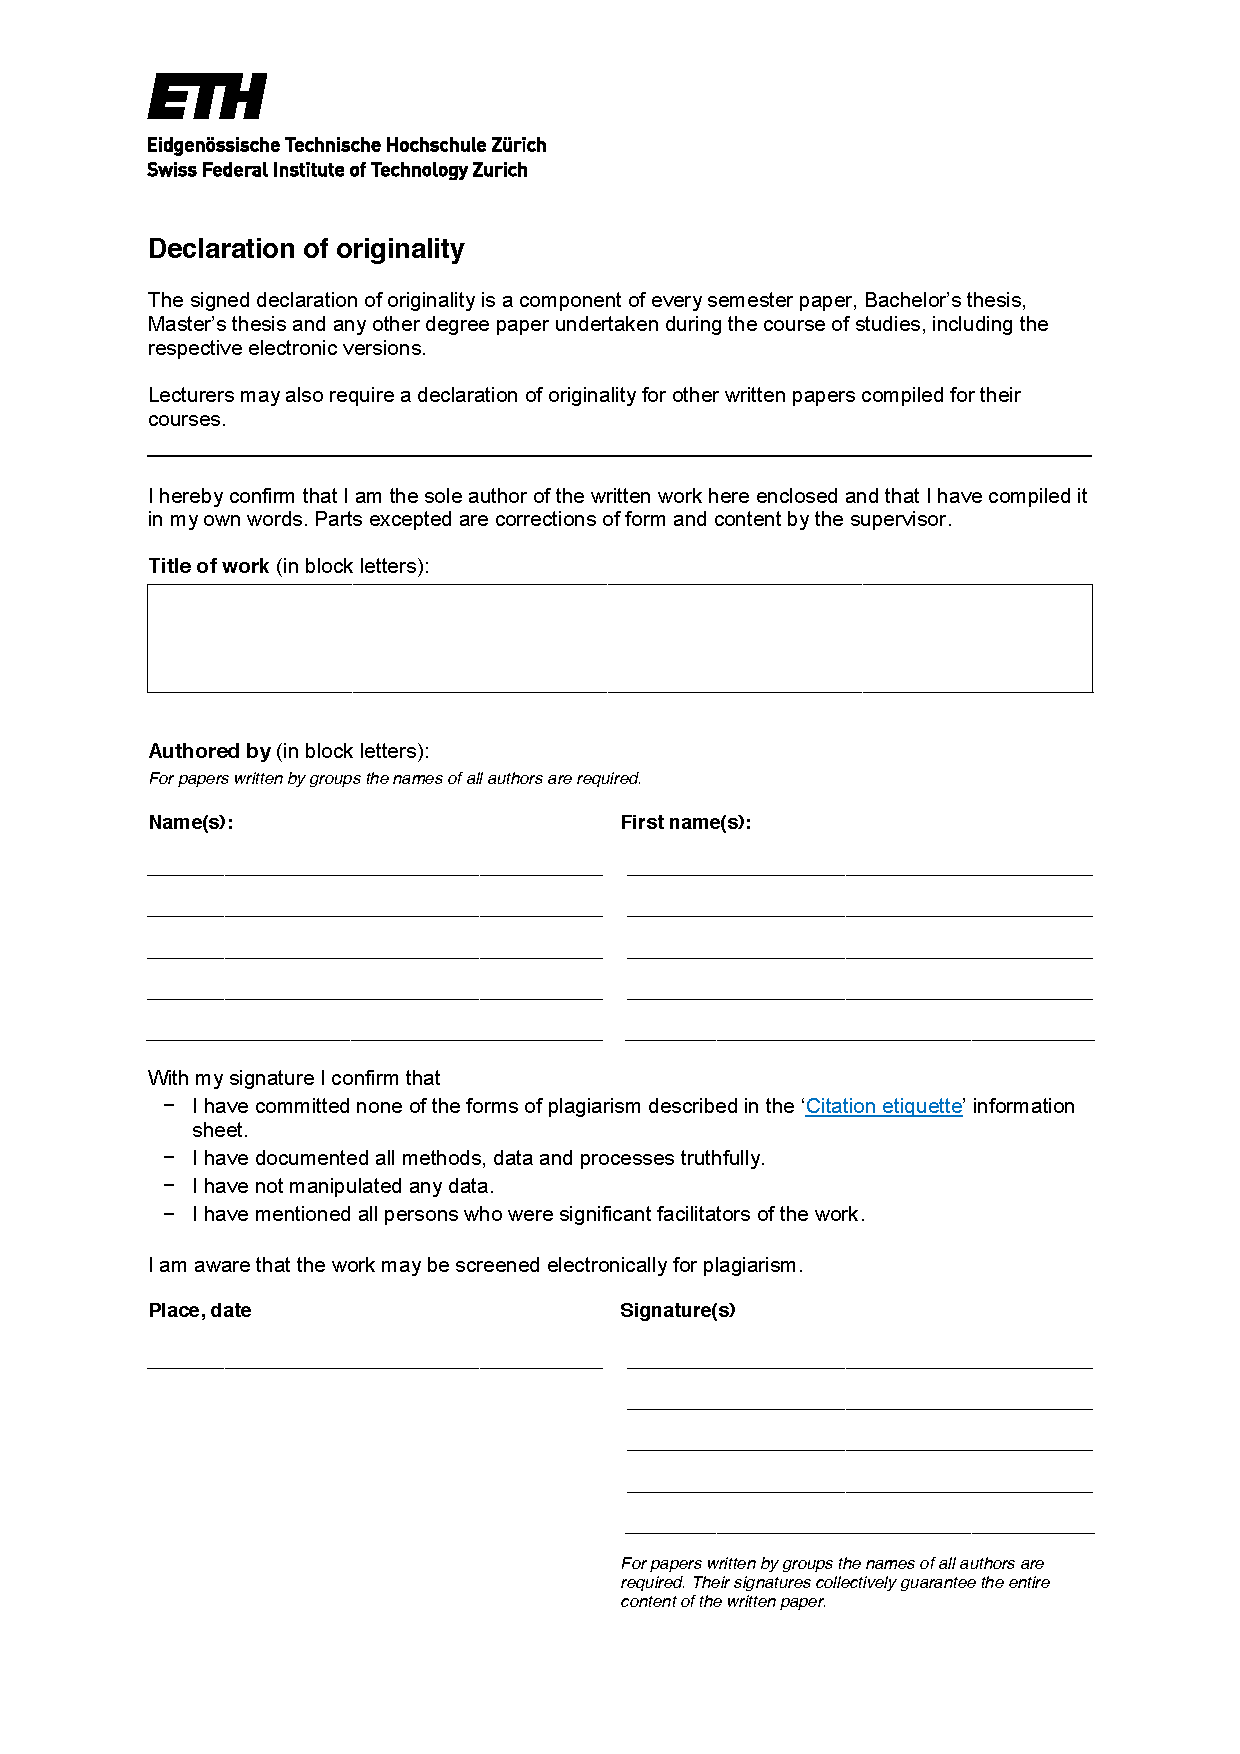
\includepdf[pages={-}]{declaration-originality.pdf}

\end{document}
